\documentclass[10pt,usenames,dvipsnames]{beamer}
\usetheme{CambridgeUS}
%\usetheme{Boadilla}
\definecolor{myred}{RGB}{163,0,0}
%\usecolortheme[named=`blue]{structure}
\usecolortheme{dove}
\usefonttheme[]{professionalfonts}
\usepackage[english]{babel}
\usepackage{amsmath,amsfonts,amssymb}
\usepackage{xcolor}
\usepackage{tikz}
\usepackage{pgfplots}
\pgfplotsset{compat=newest,compat/show suggested version=false}
\usetikzlibrary{arrows,shapes,calc,backgrounds}
\usepackage{bm}
\usepackage{textcomp}
\usepackage{gensymb}
\usepackage{verbatim}
\usepackage{paratype}
\usepackage{mathpazo}
\usepackage{listings}
\usepackage{csvsimple}

\newcommand{\cov}{\mathsf{cov}}
\newcommand{\corr}{\mathsf{corr}}
\newcommand{\var}{\mathsf{Var}}
\newcommand{\plim}{\mathrm{plim\ }}
\newcommand{\E}{\mathsf{E}}
\newcommand{\Est}{\mathsf{Est.Var}}
\newcommand{\Asy}{\mathsf{Asy.Var}}
\newcommand{\Esta}{\mathsf{Est.Asy.Var}}
\newcommand{\tr}{\mathrm{tr}}
\newcommand{\Prob}{\mathrm{Prob}}
\newcommand{\Med}{\mathsf{Med}}
\newcommand{\rank}{\mathsf{rank}}
\newcommand{\argmin}{\mathsf{arg\,min}}

\newcommand{\cc}[1]{\texttt{\textcolor{blue}{#1}}}

\definecolor{ttcolor}{RGB}{0,0,1}%{RGB}{163,0,0}

% Number theorem environments
\setbeamertemplate{theorem}[ams style]
\setbeamertemplate{theorems}[numbered]

% Reset theorem-like environments so that each is numbered separately
\usepackage{etoolbox}
\undef{\definition}
\theoremstyle{definition}
\newtheorem{definition}{\translate{Definition}}

\definecolor{ttcolor}{RGB}{0,0,1}%{RGB}{163,0,0}
\definecolor{mygray}{RGB}{248,249,250}

% Change colours for theorem-like environments
\definecolor{mygreen1}{RGB}{0,96,0}
\definecolor{mygreen2}{RGB}{229,239,229}
\setbeamercolor{block title}{fg=white,bg=mygreen1}
\setbeamercolor{block body}{fg=black,bg=mygreen2}

\lstdefinestyle{numbers}{numbers=left, stepnumber=1, numberstyle=\tiny, numbersep=10pt}
\lstdefinestyle{MyFrame}{backgroundcolor=\color{yellow},frame=shadowbox}

\lstdefinestyle{rstyle}%
{language=R,
	basicstyle=\footnotesize\ttfamily,
	backgroundcolor = \color{mygray},
	commentstyle=\slshape\color{green!50!black},
	keywordstyle=\bfseries\color{blue!50!black},
	identifierstyle=\color{blue},
	stringstyle=\color{orange},
	%escapechar=\#,
	rulecolor = \color{mygray}, 
	showstringspaces = false,
	showtabs = false,
	tabsize = 2,
	emphstyle=\color{red},
	frame = single} 

\setbeamertemplate{navigation symbols}{}

\lstset{language=R,frame=single}

\AtBeginSection{\frame{\sectionpage}}

% Remove Section 1, Section 2, etc. as titles in section pages
\defbeamertemplate{section page}{mine}[1][]{%
	\begin{centering}
		{\usebeamerfont{section name}\usebeamercolor[fg]{section name}#1}
		\vskip1em\par
		\begin{beamercolorbox}[sep=12pt,center]{part title}
			\usebeamerfont{section title}\insertsection\par
		\end{beamercolorbox}
	\end{centering}
} 

\setbeamertemplate{section page}[mine]  

\hypersetup{colorlinks, urlcolor=blue, linkcolor = myred}  

\title{R406: Applied Economic Modelling with Python}
\subtitle{Topic 15: \textcolor{myred}{Difference Equations of Second and Higher Order}}
\author{Kaloyan Ganev}

\date{2021/2022} 

\begin{document}
\maketitle

\begin{frame}[fragile]
\frametitle{Lecture Contents}
\tableofcontents
\end{frame}

\section{Introduction}
\begin{frame}[fragile]
\frametitle{Introduction}
\begin{itemize}
	\item Dependence on past or future values is not limited to one period only in the general case
	\item We first review second-order difference equations using our knowledge on how to solve a quadratic equation by hand
	\item Then we'll generalize to higher order
\end{itemize}
\end{frame}

\section{Second-order difference equations}
\begin{frame}[fragile]
\frametitle{Second-order difference equations}
\begin{itemize}
	\item The general form of second-order difference equations is:
	\[
		y_{t+2} = f(t, y_{t}, y_{t+1}),\quad t = 0,1,2,\ldots
	\]
	\item There are infinitely many solutions to this equation if no other information is supplied
	\item Let the first two values of $y_{t}$ ($y_{0}$ and $y_{1}$) be fixed and known
	\item Then $y_{0}$ and $y_{1}$ uniquely determine the solution
\end{itemize}
\end{frame}

\begin{frame}[fragile]
\frametitle{Linear equations}
\begin{itemize}
	\item The general form of a linear second-order difference equation is:
	\[
		y_{t+2} + a_{t}y_{t+1} + b_{t}y_{t} = c_{t} \quad (*)
	\]
	where $a_{t},b_{t}$, and $c_{t}$ are known (given) functions of $t$
	\item If $c_{t} = 0$ then the equation is \textbf{homogeneous}:
	\[
		y_{t+2} + a_{t}y_{t+1} + b_{t}y_{t} = 0 \quad (**)
	\]
\end{itemize}
\end{frame}

\begin{frame}[fragile]
\frametitle{Two theorems}
\begin{theorem}
	The solution of the homogeneous equation $(**)$ is:
	\[
		y_{t} = Au_{t}^{(1)} + Bu_{t}^{(2)}
	\]
	
	where $u_{t}^{(1)}$ and $u_{t}^{(2)}$ are two linearly independent solutions and $A$ and $B$ are arbitrary constants.
\end{theorem}
\end{frame}

\begin{frame}[fragile]
\frametitle{Two theorems (2)}
\begin{theorem}
	The solution of the non-homogeneous equation $(*)$ is:
	\[
		y_{t} = Au_{t}^{(1)} + Bu_{t}^{(2)} + u_{t}^{*}
	\]
	
	where $Au_{t}^{(1)} + Bu_{t}^{(2)}$ is the general solution to $(**)$ and $u_{t}^{*}$ is any particular solution of $(*)$.
\end{theorem}

\begin{itemize}
	\item There is no universal method of finding two linearly independent solutions to the non-homogeneous equation
	\item However, if we manage to find two linearly independent solutions to the homogeneous solution, then we are able to also find the general solution to $(*)$
\end{itemize}
\end{frame}

\begin{frame}[fragile]
\frametitle{Constant coefficients}
\begin{itemize}
	\item Take $(**)$ and let $a_{t} = a$ and $b_{t} = b \neq 0$ be arbitrary constants
	\item This makes the equation a constant-coefficients one:
	\[
		y_{t+2} + ay_{t+1} + by_{t} = 0
	\]
	\item Note first that if we set $y_{t} = e^{rt}$, then we would have $y_{t+1} = e^{r(t+1)} = e^{rt}e^{r}$ and $y_{t+2} = e^{r(t+2)} = e^{rt}e^{2r}$
	\item Plug these expressions in the equation:
	\[
		e^{rt}e^{2r} + ae^{rt}e^{r} + be^{rt} = 0
	\]
	\item This can also be written as:
	\[
		e^{rt}(e^{2r} + ae^{r} + b) = 0
	\] 
\end{itemize}
\end{frame}

\begin{frame}[fragile]
\frametitle{Constant coefficients (2)}
\begin{itemize}
	\item $e^{rt}$ is always positive, so we can divide both sides by it to get:
	\[
		e^{2r} + ae^{r} + b = 0
	\]
	\item If we put $m = e^{r}$, then we need to solve practically the following quadratic equation:
	\[
		m^{2} + am + b = 0
	\]
	\item This is the \textbf{characteristic equation} of the difference equation
	\item Its solutions will provide us with the values of $m$ that make $e^{rt}$ also a solution
\end{itemize}
\end{frame}

\begin{frame}[fragile]
\frametitle{The solutions of the characteristic equation}
\begin{itemize}
	\item Using high-school algebra, we find that the roots of the quadratic equation in our case equal:
	\[
		m_{1,2} = \frac{- a \pm \sqrt{a^{2} - 4b}}{2}
	\]
	\item Having also the necessary knowledge on complex numbers, you already know that the solutions are well defined for all values of the discriminant
	\item The solutions of the difference equation in the three possible cases for the value of the discriminant $D = a^{2} - 4b$ are given in the following Theorem
\end{itemize}
\end{frame}

\begin{frame}[fragile]
\frametitle{The solutions of the characteristic equation (2)}
\begin{theorem}
	The general solution of $(**)$ when $b \neq 0$ is as follows:
	\begin{enumerate}
	 	\item If $D > 0$ (two distinct real roots of the characteristic equation) then:
	 	\[
	 		y_{t} = A m_{1}^{t} + B m_{2}^{t}, \quad m_{1,2} = \frac{- a \pm \sqrt{a^{2} - 4b}}{2}
	 	\]
	 	\item If $D = 0$ (one double real root) then:
	 	\[
	 		y_{t} = (A + Bt) m^{t}, \quad m = -\frac{a}{2}
	 	\]
	 	\item If $D < 0$ (two complex conjugate roots) then:
	 	\[
	 		y_{t} = R^{t}(A\cos(\theta t) + B\sin(\theta t)), \quad R = \sqrt{b},\, \cos(\theta) = -\frac{a}{2\sqrt{b}},\, \theta \in [0,\pi]
	 	\]
	\end{enumerate} 
\end{theorem}
\end{frame}

\begin{frame}[fragile]
\frametitle{The solutions of the characteristic equation (3)}
\begin{itemize}
	\item First, we note that we need two initial values of $y_{t}$ to solve the equation
	\item If those two values are given, say $y_{0}$ and $y_{1}$, then the constants $A$ and $B$ are uniquely determined
	\item In the case when the solutions are complex conjugates, the fact that they contain sines and cosines implies that they characterize cyclical behaviour (oscillations)
	\item The value of the radius (modulus) $R$ determines the type of cyclical fluctuations:
	\begin{enumerate}
		\item When $|R| < 1$, the oscillations are damped (their amplitude decreases over time)
		\item When $|R| > 1$, the oscillations are explosive (increasing amplitude)
		\item $|R| = 1$, oscillations remain with unchanged amplitude over time
	\end{enumerate}
\end{itemize}
\end{frame}

\begin{frame}[fragile]
\frametitle{The non-homogeneous case}
\begin{itemize}
	\item General form:
	\[
		y_{t+2} + a y_{t+1} + b y_{t} = c_{t}, \quad b \neq 0 \quad (\spadesuit)
	\]
	\item Recall that according to Theorem 2 the solution is:
	\[
		y_{t} = Au_{t}^{(1)} + Bu_{t}^{(2)} + u_{t}^{*}
	\]
	where $u_{t}^{*}$ is a particular solution of ($\spadesuit$)
	\item It turns out that finding $u_{t}^{*}$ is a very difficult task even if $c_{t}$ is a relatively simple function
\end{itemize}
\end{frame}

\begin{frame}[fragile]
\frametitle{The non-homogeneous case (2)}
\begin{itemize}
	\item An easier case: $c_{t} = c$, i.e. a constant
	\item Then ($\spadesuit$) becomes: 
	\[
		y_{t+2} + a y_{t+1} + b y_{t} = c, \quad b \neq 0 \quad (\heartsuit)
	\]
	\item So, we have to find a solution of the form: $y_{t} = C$, where $C = const$
	\item If $y_{t} = C$, then $y_{t+1} = y_{t+2} = C$. Substitute all these in $(\heartsuit)$ to get:
	\[
		C + a C + b C = c \Leftrightarrow C(1 + a + b) = c
	\]
	\item Therefore, if $1 + a + b \neq 0$:
	\[
		C = \frac{c}{1 + a + b} 
	\]
	\item Then, the particular solution is:
	\[
		u_{t}^{*} = \frac{c}{1 + a + b}
	\]
\end{itemize}
\end{frame}

\begin{frame}[fragile]
\frametitle{The non-homogeneous case (3)}
\begin{itemize}
	\item What if $1 + a + b = 0$?
	\item Then there is no constant function that can satisfy $(\heartsuit)$
	\item In such a case we can write $b = -(1 + a)$ and substitute this in $(\heartsuit)$:
	\[
		y_{t+2} + a y_{t+1} - (1 + a) y_{t} = c
	\]
	\item In this case, a constant function would solve only the homogeneous function, so we look for another particular solution
\end{itemize}
\end{frame}

\begin{frame}[fragile]
\frametitle{The non-homogeneous case (4)}
\begin{itemize}
	\item Try with $u_{t}^{*} = Dt$:
	\[
	\begin{array}{lcl}
		u_{t+2}^{*} + a u_{t+1}^{*} - (1 + a) u_{t}^{*} & = & D(t+2) + a D(t+1) - (1 + a)Dt = \\
		\quad\\
		& = & Dt + 2D + aDt + aD - Dt - aDt = \\
		\quad\\
		& = & (a + 2)D
	\end{array}
	\]
	\item So, if $a \neq -2$, then $\displaystyle D = \frac{c}{a + 2}$, and the particular solution is:
	\[
		u_{t}^{*} = \frac{c t}{a + 2}
	\]
	
\end{itemize}
\end{frame}

\begin{frame}[fragile]
\frametitle{The non-homogeneous case (5)}
\begin{itemize}
	\item Now, what if in addition to $1 + a + b = 0$ we have also $a = -2$? Then $(\heartsuit)$ becomes:
	\[
		y_{t+2} - 2y_{t+1} + y_{t} = c
	\]
	\item We try then to find a solution of the form $u_{t}^{*} = Dt^{2}$. With this, we have:
	\[
	\begin{array}{lcl}
		u_{t+2}^{*} - 2 u_{t+1}^{*} + u_{t}^{*} & = & D(t+2)^{2} - 2 D(t+1)^{2} + Dt^{2} = \\
		\quad\\
		& = & Dt^{2} + 4Dt + 4D - 2Dt^{2} - 4Dt - 2D + Dt^{2} = \\
		\quad\\
		& = & \displaystyle 2D \Rightarrow D = \frac{c}{2}
	\end{array}
	\]
	\item The particular solution is:
	\[
		u_{t}^{*} = \frac{c t^{2}}{2}
	\]
\end{itemize}
\end{frame}

\begin{frame}[fragile]
\frametitle{Stability of solutions}
\begin{itemize}
	\item Generally speaking, a discrete dynamic system is \textbf{stable} if whatever changes are made to the initial conditions, eventually their effect vanishes as $t \to \infty$
	\item Otherwise (i.e. when even small changes might lead to large differences in long-term behaviour) the system is \textbf{unstable}
	\item Returning to $(\heartsuit)$, it is called \textbf{globally asymptotically stable} if the solution of its associated homogeneous equation tends to 0 as $t \to \infty$
\end{itemize}

\begin{theorem}
	The equation $(\heartsuit)$ is globally asymptotically stable iff the following two equivalent conditions are satisfied:
	\begin{itemize}
		\item[(A)] The moduli of the roots of the characteristic equation $m^{2} + am + b = 0$ are strictly lower than 1
		\item[(B)] $|a| < 1 + b$ and $|b| < 1$
	\end{itemize}
\end{theorem}
\end{frame}

\begin{frame}[fragile]
\frametitle{Proof of Theorem 4}
\begin{itemize}
	\item (This proof is provided exceptionally because the equivalence of (A) and (B) is not so obvious)
	\item We will prove first that $(B) \Rightarrow (A)$
	\item Consider first the case in which the characteristic equation has two complex conjugate roots, i.e. $\displaystyle a^2 - 4b < 0 \Leftrightarrow b > \frac{a^{2}}{4}$
	\item Note that the latter implies that $b > 0$
	\item Both roots have moduli equal to $\sqrt{b}$
	\item If $b < 1$ (and obviously $|a| < 1 + b$), then $\sqrt{b} < 1$. This proves $(B) \Rightarrow (A)$
	\item Now, in order to prove $(A) \Rightarrow (B)$, look at the following graph
\end{itemize}
\end{frame}

\begin{frame}[fragile]
\frametitle{Proof of Theorem 4 (2)}
\begin{center}
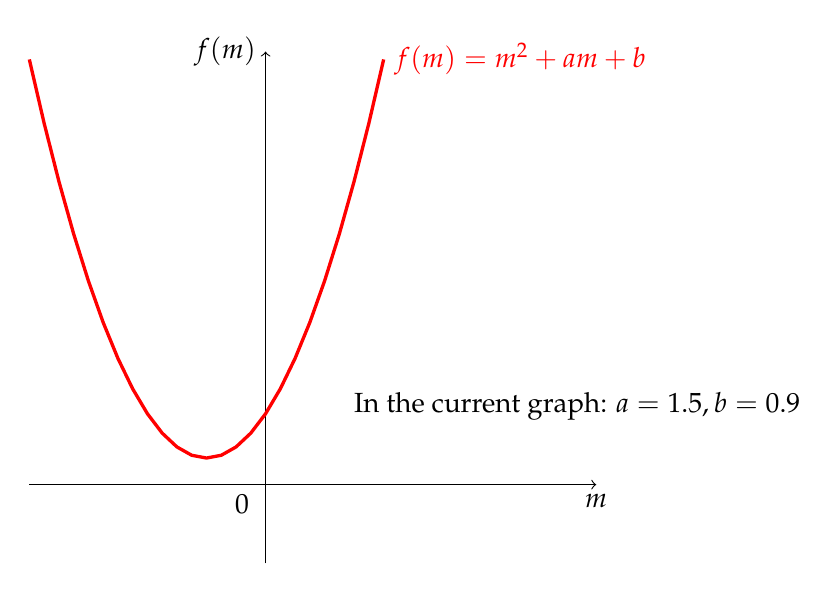
\begin{tikzpicture}[domain=-4:4]
	\draw[->] (-3,0) -- (4.2,0) node[below] {$m$};
	\draw[->] (0,-1) -- (0,5.5) node[left] {$f(m)$};
	\draw[very thick, color=red, domain = -3:1.5] plot ({\x},{\x*\x + 1.5*\x + 0.9} ) node[right] {$f(m) = m^2 + am + b$};
	\draw (-0.3,-0.5) node[above] {0}; 
	\draw (1,1) node[right] {In the current graph: $a = 1.5, b = 0.9$};
\end{tikzpicture}
\end{center} 
\end{frame}

\begin{frame}[fragile]
\frametitle{Proof of Theorem 4 (3)}
\begin{itemize}
	\item From the graph it is visible that the parabola never crosses the horizontal axis (this is the same as the fact that none of the roots is real)
	\item In other words, no matter what the value of $m$, we have $f(m) > 0$
	\item Take $m$ to equal in turns -1 and 1; then:
	\[
		\begin{array}{lcl}
			f(-1) = 1 - a + b > 0 \Rightarrow a < 1 + b\\
			f(1) = 1 + a + b > 0 \Rightarrow -a < 1 + b
		\end{array}
	\]
	\item But these two are equivalent to $|a| < 1 + b$
	\item From the fact that the moduli of the roots are strictly less than one directly follows that $\sqrt{b} < 1$, and therefore $b < 1$
	\item The above leads to $(A) \Rightarrow (B)$
	\item This completes the proof for complex roots
\end{itemize}
\end{frame}

\begin{frame}[fragile]
\frametitle{Proof of Theorem 4 (4)}
\begin{itemize}
	\item In the case of real roots, the discriminant is non-negative: $a^{2} - 4b \geq 0$
	\item This is equivalent to $\displaystyle b \leq \frac{a^{2}}{4}$
	\item The two roots are:
	\[
		m_{1,2} = \frac{-a \pm \sqrt{a^{2} - 4b}}{2}
	\]
	\item In the real case, that their moduli are strictly less than 1 means that their absolute values should be less than 1
	\item For $m_{1}$ this means (check that the same result is obtained for $m_{2}$):
	\[
		-1 < \frac{-a + \sqrt{a^{2} - 4b}}{2} < 1 \Rightarrow -2 + a < \sqrt{a^{2} - 4b} < 2 + a
	\]	
\end{itemize}
\end{frame}

\begin{frame}[fragile]
\frametitle{Proof of Theorem 4 (5)}
\begin{itemize}
	\item Square all parts of the last double inequality to get:
	\[
		a^{2} - 4a + 4 < a^{2} - 4b < a^{2} + 4a + 4, 
	\]
	or:
	\[
		- a + 1 < - b < a + 1,
	\]
	or:
	\[
		- a < b + 1 < a,
	\]
	which is the same as $|a| < b + 1$
	\item The latter can also be obtained from the fact that $f(-1) > 0$ and $f(1) > 0$
	
\end{itemize}
\end{frame}

\begin{frame}[fragile]
\frametitle{Proof of Theorem 4 (6)}
\begin{itemize}
	\item Note also that in those two points the signs of the first derivative of $f(m)$, $f'(m) = 2m + a$, are known:
	\[
		\begin{array}{lcl}
			f'(-1) = -2 + a < 0\\
			f'(1) = 2 + a > 0
		\end{array}
	\]
	\item From the latter follows that $|a| < 2$
	\item Combine this with $\displaystyle b \leq \frac{a^{2}}{4}$ to find that:
	\[
		b \leq \frac{a^{2}}{4} < \frac{4}{4} = 1
	\]
	\item This proves $(A) \Rightarrow (B)$
\end{itemize}
\end{frame}

\begin{frame}[fragile]
\frametitle{Proof of Theorem 4 (7)}
\begin{center}
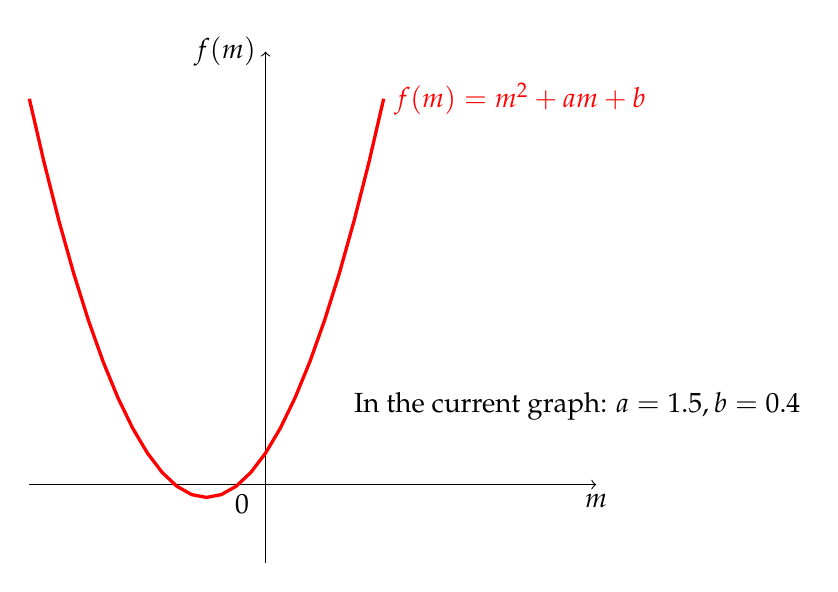
\begin{tikzpicture}[domain=-4:4]
	\draw[->] (-3,0) -- (4.2,0) node[below] {$m$};
	\draw[->] (0,-1) -- (0,5.5) node[left] {$f(m)$};
	\draw[very thick, color=red, domain = -3:1.5] plot ({\x},{\x*\x + 1.5*\x + 0.4} ) node[right] {$f(m) = m^2 + am + b$};
	\draw (-0.3,-0.5) node[above] {0}; 
	\draw (1,1) node[right] {In the current graph: $a = 1.5, b = 0.4$};
\end{tikzpicture}
\end{center} 
\end{frame}

\begin{frame}[fragile]
\frametitle{Proof of Theorem 4 (8)}
\begin{itemize}
	\item To prove equivalence in the reverse direction, first note that if $|a| < 1 + b$ and $b < 1$, obviously $|a| < 2$
	\item The latter is equivalent to $-2 < a < 2$, or $2 + a > 0$ and $-2 + a < 0$
	\item We can also see that $2 + a$ and $-2 + a$ are the values of $f'(m)$ respectively at 1 and -1
	\item Using $|a| < 1 + b$, we can consecutively write:
	\[
		\begin{array}{lcl}
			-a < 1 + b < a & \Leftrightarrow & -a + 1 < -b < a + 1 \Leftrightarrow \\
			& \Leftrightarrow & -4a + 4 < -4b < 4a + 4 \Leftrightarrow\\
			& \Leftrightarrow & a^{2} - 4a + 4 < a^{2} - 4b < a^{2} + 4a + 4 \Leftrightarrow\\
			& \Leftrightarrow & (a - 2)^{2} < a^{2} - 4b < (a + 2)^{2} 			
		\end{array}
	\]
	\item From this point onwards, establishing that the roots of the characteristic equation lie in $(-1,1)$ is straightforward
\end{itemize}
\end{frame}

\begin{frame}[fragile]
\frametitle{Example: The multiplier-accelerator model}
\begin{itemize}
	\item Keynesian business cycle model, due to Samuelson (1939)
	\item We consider a slightly modified version
	\item Model equations:
	\[
		\begin{array}{lcl}
			C_{t} & = & a + bY_{t-1}\\
			I_{t} & = & v(Y_{t-1} - Y_{t-2})\\
			G_{t} & = & \overline{G}, \quad \forall t\\
			E_{t} & = & C_{t} + I_{t} + G_{t}\\
			Y_{t} & = & E_{t}
		\end{array}
	\]
	\item Combine all equations to get the following second-order non-homogeneous difference equation:
	\[
		Y_{t} - (b + v)Y_{t-1} + vY_{t-2} = a + \overline{G}
	\]
\end{itemize}
\end{frame}

\begin{frame}[fragile]
\frametitle{Example: The multiplier-accelerator model (2)}
\begin{itemize}
	\item To find a particular solution, set $Y_{t} = Y^{*} = const$, i.e.:
	\[
		Y^{*} - (b + v)Y^{*} + vY^{*} = a + \overline{G}
	\]
	\item After rearrangement, we have:
	\[
		Y^{*} = \frac{a + \overline{G}}{1-b}
	\]
	\item The latter is interpreted in the following way: equilibrium income corresponds to the result from the simple Keynesian multiplier model
\end{itemize}
\end{frame}

\begin{frame}[fragile]
\frametitle{Example: The multiplier-accelerator model (3)}
\begin{itemize}
	\item The homogeneous equation that corresponds to this example is:
	\[
		Y_{t} - (b + v)Y_{t-1} + vY_{t-2} = 0
	\]
	\item The roots of its characteristic equation are as follows:
	\[
		m_{1,2} = \frac{(b+v) \pm \sqrt{(b+v)^{2} - 4v}}{2}
	\]
	\item Three cases emerge again:
	\begin{enumerate}
		\item Two distinct real roots
		\item One double real root
		\item Two complex conjugate roots
	\end{enumerate}
\end{itemize}
\end{frame}

\begin{frame}[fragile]
\frametitle{Example: The multiplier-accelerator model (4)}
\begin{itemize}
	\item \textcolor{red}{Case 1:} Two distinct real roots, i. e. $(b+v)^{2} - 4v > 0$ 
	\item In order to be able to analyse the dynamics implied by the difference equation, it is a good idea to use the Vieta formulae which define the relationships between the two roots:
	\[
		\begin{array}{lcl}
			m_{1} + m_{2} & = & b + v\\
			m_{1}m_{2} & = & v
		\end{array}
	\]
	\item We can use these two to find that:
	\[
	\begin{array}{lcl}
		(1 - m_{1})(1 - m_{2}) & = & 1 - m_{2} - m_{1} + m_{1}m_{2} = \\
		& = & 1 - (b + v) + v = \\
		& = & 1 - b
	\end{array}
	\]
	\item As $b$ is interpreted as MPC, $b \in (0,1)$. The latter implies that also $(1 - m_{1})(1 - m_{2}) \in (0,1)$
\end{itemize}
\end{frame}

\begin{frame}[fragile]
\frametitle{Example: The multiplier-accelerator model (5)}
\begin{itemize}
	\item In this case, the general solution is given by:
	\[
		Y_{t} = Am_{1}^{t} + Bm_{2}^{t} + Y^{*}
	\]
	\item The larger of the two roots (say this is $m_{1}$ in our example) determines the development path of $Y_{t}$\footnote{This is valid in general for any polynomial: the root having the largest modulus dominates the remaining ones.}
	\item From $b > 0$ and $v > 0$ follows that $m_{1}m_{2} = v > 0$; this implies that $m_{1}$ and $m_{2}$ should either be both positive or both negative
	\item But because of the fact that $m_{1} + m_{2} = b + v > 0$, the option that the two roots are both negative is ruled out; therefore $m_{1} > 0$ and $m_{2} > 0$
	\item This means that $Y_{t}$ is not characterized with oscillations
	\item Two possibilities arise with respect to the magnitude of the larger root 
\end{itemize}
\end{frame}

\begin{frame}[fragile]
\frametitle{Example: The multiplier-accelerator model (6)}
\begin{itemize}
	\item If \textcolor{mygreen1}{$m_{1} > 1$}, then we should also have $m_{2} > 1$ (otherwise the condition $(1 - m_{1})(1 - m_{2}) \in (0,1)$ will be violated)
	\item With $m_{1} > m_{2} > 1$, $Y_{t}$ has an explosive path
	\item The above also implies that $m_{1}m_{2} = v > 1$, i. e. the accelerator coefficient is greater than 1
	\item If \textcolor{mygreen1}{$m_{1} < 1$}, then $0 < m_{2} < m_{1} < 1$. From this follows first that $v \in (0,1)$ and second, that the dynamics is damped towards the equilibrium
	\item \textcolor{orange}{Note that the roots cannot equal 1 since otherwise $(1 - m_{1})(1 - m_{2})$ would not be positive but would also equal zero!}
\end{itemize}
\end{frame}

\begin{frame}[fragile]
\frametitle{Example: The multiplier-accelerator model (7)}
\begin{itemize}
	\item \textcolor{red}{Case 2:} One double real root, i. e. $(b+v)^{2} - 4v = 0$
	\item The root equals:
	\[
		m_{1,2} = \frac{b + v}{2} = m
	\]
	\item Since $m^{2} = v$, we have $v \geq 0$; but $m$ cannot be zero because $b > 0$, therefore $v > 0$ (although this should be an obvious assumption from the very beginning); finally, this means that $m > 0$
	\item Again, two possibilities
	\item First, if $0 < m < 1$, then we should have $0 < v < 1$ and a damped path for income
	\item Second, if $m > 1$, then $v > 1$ and the dynamics of $Y_{t}$ is explosive
	\item \textcolor{orange}{By the same reasoning as above, $m$ cannot be equal to one} 
\end{itemize}
\end{frame}

\begin{frame}[fragile]
\frametitle{Example: The multiplier-accelerator model (8)}
\begin{itemize}
	\item \textcolor{red}{Case 3:} Two complex conjugate roots, i. e. $(b+v)^{2} - 4v < 0$
	\item The roots equal:
	\[
		\begin{array}{lcl}
			m_{1} = \alpha + i\beta\\
			m_{2} = \alpha - i\beta\\
		\end{array}
	\]
	where $\displaystyle \alpha = \frac{b+v}{2}$ and $\displaystyle \beta = \frac{\sqrt{4v - (b + v)^{2}}}{2}$
	\item The general  solution to the difference equation is:
	\[
		Y_{t} = R^{t}[A\cos(\theta t) + B\sin(\theta t)] + Y^{*},
	\]
	where $\displaystyle R = \sqrt{\alpha^{2} + \beta^{2}} = \sqrt{\frac{(b + v)^{2} + 4v - (b + v)^{2}}{4}} = \sqrt{v}$, $\displaystyle \cos(\theta) = \frac{b + v}{2\sqrt{v}}$, and $\displaystyle \sin(\theta) = \frac{\sqrt{4v - (b + v)^{2}}}{2\sqrt{v}}$
\end{itemize}
\end{frame}

\section{Higher-order equations}
\begin{frame}[fragile]
\frametitle{Higher-order equations}
\begin{itemize}
	\item In general, we can have $p$th-order difference equations
	\[
		y_{t+p} = f(t, y_{t}, y_{t+1}, \ldots, y_{t+p-1}), \quad t = 0, 1, 2, \ldots
	\]
	\item In order to have a uniquely defined solution, $p$ initial values are needed
	\item The general solution of such an equation is a function $y_{t} = g(t;C_{1},\ldots, C_{p})$, where $C_{1}, \ldots, C_{p}$ are arbitrary constants
	\item For each given set of values of $C_{1}, \ldots, C_{p}$, we can obtain the corresponding solution of the equation
\end{itemize}
\end{frame}

\begin{frame}[fragile]
\frametitle{Higher-order equations: The linear case}
\begin{theorem}
	The  $p$th-order linear homogeneous difference equation:
	\[
		y_{t+p} + a_{1}(t)y_{t+p-1} + \ldots + a_{p-1}(t)y_{t+1} + a_{p}(t)y_{t} = 0, \quad a_{p}(t) \neq 0
	\]
	has the following solution:
	\[
		y_{t} = C_{1}u_{t}^{(1)} + \ldots + C_{p}u_{t}^{(p)}
	\]
	where $u_{t}^{(1)}, \ldots, u_{t}^{(p)}$ are $p$ linearly independent solutions of the characteristic equation, and $C_{1}, \ldots, C_{p}$ are arbitrary constants.
\end{theorem}
\end{frame}

\begin{frame}[fragile]
\frametitle{Higher-order equations: The linear case (2)}
\begin{theorem}
	The  $p$th-order linear non-homogeneous difference equation:
	\[
		y_{t+p} + a_{1}(t)y_{t+p-1} + \ldots + a_{p-1}(t)y_{t+1} + a_{p}(t)y_{t} = b_{t}, \quad a_{p}(t) \neq 0
	\]
	has the following solution:
	\[
		y_{t} = C_{1}u_{t}^{(1)} + \ldots + C_{p}u_{t}^{(p)} + u_{t}^{*}
	\]
	where $C_{1}u_{t}^{(1)} + \ldots + C_{p}u_{t}^{(p)}$ is the general solution of the homogeneous equation, and $u_{t}^{*}$ is a particular solution of the non-homogeneous equation
\end{theorem}
\end{frame}

\begin{frame}[fragile]
\frametitle{Linear higher-order equations with constant coefficients}
\begin{itemize}
	\item Homogeneous case:
	\[
		y_{t+p} + a_{1}y_{t+p-1} + \ldots + a_{p-1}y_{t+1} + a_{p}y_{t} = 0, \quad t = 0, 1, 2, \ldots
	\]
	\item Non-homogeneous case:
	\[
		y_{t+p} + a_{1}y_{t+p-1} + \ldots + a_{p-1}y_{t+1} + a_{p}y_{t} = b_{t}, \quad t = 0, 1, 2, \ldots
	\]
	\item Solutions having the form $y_{t} = m^{t}$ are sought, as we did in the second-order equations case
	\item This leads to the following characteristic equation:
	\[
		m^{p} + a_{1}m^{p-1} + \ldots + a_{p-1}m + a_{p} = 0
	\]
	
\end{itemize}
\end{frame}

\begin{frame}[fragile]
\frametitle{Linear higher-order equations with constant coefficients (2)}
\begin{itemize}
	\item This is a polynomial equation, and it has as many roots as the degree of the polynomial ($p$ in the current case)
	\item Those $p$ roots can either be different, or there could be multiple roots (as with double roots in second-order equations)
	\item Also, there could be complex roots, and they always come in pairs of conjugates
\end{itemize}
\end{frame}

\begin{frame}[fragile]
\frametitle{Linear higher-order equations with constant coefficients (3)}
The general rules that are followed in finding the roots are as follows:
	\begin{enumerate}
		\item If a real root $m_{i}$ is unique, then it provides one solution $m_{i}^{t}$
		\item If a real root $m_{j}$ is repeated $k$ times, then it provides $k$ solutions $m_{j}^{t}, tm_{j}^{t}, t^{2}m_{j}^{t},\ldots,t^{k-1}m_{j}^{t}$
		\item A pair of complex conjugates  $\alpha \pm i\beta$ which is encountered only once among the list of roots provides two solutions: $R^{t}\cos(\theta t)$ and $R^{t}\sin(\theta t)$
		\item A pair of complex conjugates  $\alpha \pm i\beta$ which is encountered $l$ times among the list of root provides $2l$ solutions: $u, v, tu, tv,, \ldots, t^{l-1}u, t^{l-1}v$, where  $u = R^{t}\cos(\theta t)$ and $v = R^{t}\sin(\theta t)$
	\end{enumerate}
	\textcolor{orange}{For the non-homogeneous equation, a particular solution $u_{t}^{*}$ needs also to be found.}
\end{frame}

\begin{frame}[fragile]
\frametitle{Stability conditions for higher-order equations}
\begin{theorem}
	A necessary and sufficient condition for the $p$th order linear difference equation is that the roots of the characteristic polynomial all lie within the unit circle, i. e. all have moduli less than 1.
\end{theorem}
\end{frame}

\begin{frame}[fragile]
\frametitle{References}
\begin{itemize}
	\item Chiang, A. and K. Wainwright (2005): \emph{Fundamental Methods of Mathematical Economics}, McGraw-Hill, Ch. 18
	\item Elaydi, S. (2005): \emph{An Introduction to Difference Equations}, Springer, Ch. 1
	\item Shone, R. (2002): \emph{Economic Dynamics: Phase Diagrams and Their Economic Application}, Cambridge University Press, Ch. 3
	\item Syds\ae ter, K., P. Hammond, and A. Str\o m (2008): \emph{Further Mathematics for Economic Analysis}, Prentice Hall, Ch.11
\end{itemize}
\end{frame}

\end{document}
	


